\documentclass[12pt]{article}
\usepackage{amsfonts}
\usepackage{amsmath}
\usepackage{graphicx} 
\usepackage{float}
\usepackage[margin=1in]{geometry}
\usepackage[caption = false]{subfig}
\usepackage{/Users/timbarry/Documents/optionFiles/mymacros}
\usepackage[toc,page]{appendix}
\usepackage[
backend=biber,
style=authoryear,
maxcitenames=2,
maxbibnames=6,
backref=true,
doi=false,
isbn=false,
url=false,
eprint=false
]{biblatex}
\addbibresource{/Users/timbarry/optionFiles/Proposal.bib}
\newtheorem{proposition}{Proposition}
\allowdisplaybreaks

\begin{document}

\begin{center}
\textbf{Stats paper proposal} \\
Tim B
\end{center}

In this document I chart out several ideas for a next statistics paper. The following keywords are relevant: randomization tests, conditional randomization/permutation tests, $e$-values, multiple hypothesis testing, sample splitting, robustness, and online learning. I propose two main directions and a few tertiary directions. I also suggest a CRISPR genomics application.

\section*{Direction 1: A more general framework for randomization tests}

\subsection*{Motivation and background}

Randomization tests are tests in which a statistic is recomputed over permuted, resampled, rotated, or otherwise transformed versions of the data to produce an empirical null distribution against which a statistic computed on the raw data is compared. Randomization tests are ubiquitous throughout all of statistics and science. For example, randomization tests routinely are used in genetics to assess the association of SNPs (\cite{Johnson2010}) and to test the differential expression of genes (\cite{Maleki2020}) and in neuroscience to improve the robustness of GLMs in the analysis of brain imaging data (\cite{Winkler2014}). % See \cite{Dobriban2021} for a recent review and unifying theoretical analysis of randomization tests.
Despite their widespread popularity, randomization tests pose several practical challenges, especially in high-multiplicity settings: miscalibrated $p$-values can cause type-I error inflation; combining $p$-values across many hypothesis tests can result in excessively conservative or liberal discovery sets, especially when tests are dependent; and sample splitting -- a procedure required by certain randomization tests, such as the recently-proposed, ML-based holdout randomization test (\cite{Tansey2021a}) -- can result in non-reproducible $p$-values.

Building closely on the work of several authors (\cite{Wang2020b,Vovk2020,Vovk2021b}), we propose a simple new framework for randomization testing that helps to resolve these challenges. The framework leverages $e$-values, test statistics that by definition are nonnegative and have (at most) unit expectation under the null. We capture the standard, $p$-value based approach to randomization testing a special case of our framework. Although the theory applies broadly, we focus mostly on (marginal) permutation tests, conditional randomization tests, and conditional permutation tests as illustrative examples.

As a brief review, let $T^*$ be the test statistic computed on the raw data, and let $T_1, T_2 \dots, T_B$ be the test statistics recomputed on the permuted (or resampled, etc.) data. We assume for simplicity that there are no ties among the $T_i$s, although this assumption has minimal impact on the theory.  Randomization tests satisfy the following key invariance property: the vector $(T^*, T_1, T_2, \dots, T_B)$ is \textit{exchangeable} under the null hypothesis. This means that the cumulative distribution function of $(T^*, T_1, T_2, \dots, T_B)$ is invariant to permutations. Exchangeability implies that the empirical $p$-value
$$ p_B =  \frac{\sum_{i=1}^B \mathbb{I}\left(T^* \leq T_i \right) }{B}$$ is valid, i.e., $p$ stochastically dominates the uniform distribution. (One often adds a $1$ to both the numerator and denominator to ensure finite-sample correctness, but for large $B$, the two expressions coincide almost exactly.) The standard practice is to reject the null hypothesis at level $\alpha \in (0,1)$ if $p < \alpha$, adjusting for multiple testing (typically via BH) to control FDR in high multiplicity settings.

\subsection*{Linear $e$-values}

We propose a more general framework for randomization testing based on $e$-values. For $i \in \{1, \dots, B\}$, let $T_{(1)}, \dots, T_{(B)}$ be the order statistics of  $T_1, \dots, T_B$. Define $I_i = \mathbb{I}(T^* \leq T_{(i)}).$ For given constants $a_0, a_1, \dots, a_B \in \R$, define the test statistic $e$ by 
\begin{equation}\label{lin_e_def}
e = a_0 + \sum_{i=1}^B a_i I_i,
\end{equation}
 where $e$ is a nonnegative random variable such that $\E[e] = 1$ under the null hypothesis. We call $e$ a ``linear $e$-value'' so as to distinguish it from other, more general $e$-values. We state two key propositions that enable us to construct linear $e$-values with ease. The first proposition derives the expectation of $I_i$ under the null hypothesis by applying a well-known fact about the ranks of exchangeable variables (recorded in \cite{Kuchibhotla2020}).

\begin{proposition}
For $i \in \{1, \dots, B\}$, $\E[I_i] = i/(B+1).$
\end{proposition}
\textbf{Proof}: The vector $(T^*, T_1, \dots, T_n)$ is exchangeable. Therefore, by Corollary 1 of (\cite{Kuchibhotla2020}),  $$\P\left[\textrm{rank}(T^*) \leq i\right] = \frac{i}{1+B},$$ where $$\textrm{rank}(T^*) = | \{ j \in \{1, \dots, B\} :  T_j \leq T^*  \} | + 1$$ is the rank of $T^*$. But $\textrm{rank}(T^*) = i$ if and only if $T^* \leq T_{(i)}$. Therefore, $\P( T^* \leq T_{(i)}) = i/(B+1)$, implying the conclusion. $\square$
\\ \\
The next proposition derives a simple expression for the $r$th power of the sum of the $I_i$s (proof deferred to appendix).
\begin{proposition}\label{thm:power_of_is}
For $r,B \in \N,$
$$ \left(\sum_{i=1}^B I_i\right)^r = \sum_{i=1}^B \left[ (B - i + 1)^r - (B - i)^r \right] I_i.$$ Equivalently, the $r$th power of the empirical right-sided $p$-value $p_B := \frac{1}{B} \sum_{i=1}^B  I_i $ is $$ p_B^r = \sum_{i=1}^B \left[ (1 - i/B + 1/B)^r - (1 - i/B)^r \right]I_i := \sum_{i=1}^B M(B,r,i) I_i.$$ Finally, for given $x_0 \in \R$ and coefficients $c_0, c_1, \dots, c_r \in \R$, the $r$th degree polynomial $\sum_{j=0}^r c_j(p_B - x_0)^j$ is given by
$$
\sum_{j=0}^r c_j(p_B - x_0)^j = \sum_{j=0}^r c_j x_0^j(-1)^j + \sum_{i=1}^B \left[\sum_{j=1}^r \sum_{k=1}^j c_j x^{j-k}_0 \binom{j}{k}(-1)^{j-k} M(B,k,i) \right] I_i.
$$
\end{proposition}
In other words, the $r$th power of the sum of the $I_i$s is a simple linear combination of the $I_i$s, not a messy multinomial expression as one might initially expect. Equivalently, the $r$th power of the empirical right-sided $p$-value (i.e., $p_B = (1/B) \sum_{i=1}^B I_i$) is a simple linear combination of the $I_i$s. Finally, the $r$th degree polynomial of $p_B$ centered at $x_0$ with coefficients $c_0, \dots, c_r$ is a straightforward extension of the above. This result, though simple, is to the best of our knowledge new.

\subsection*{Examples of linear $e$-values}

Using the above propositions, we construct several example linear $e$-values.
\\ \\ \noindent
\textbf{Example 1: Warmup.} Setting $a_i = (B+1)/i$ and $c = 0$ in definition (\ref{lin_e_def}), we obtain
$$e = (B+1)\sum_{i=1}^B \frac{I_i}{i}.$$ The variable $e$ clearly is nonnegative. Moreover, $$ \E(e) = (B+1) \sum_{i=1}^B \frac{ i }{i(B+1)} = 1.$$ Therefore, $e$ is a linear $e$-value.
\\ \\ \noindent
\textbf{Example 2: $p^\textrm{shift}$-values.} We recover standard $p$-values (up to a translation) as a special case of the proposed framework. Set $c = 3/2$ and $a_i = -1/B$ in definition (\ref{lin_e_def}). Then we obtain
$$e = (3/2) - \frac{1}{B} \sum_{i=1}^B I_i$$
as our test statistic. This statistic clearly is nonnegative. (In fact, it is greater than or equal to $1/2$.) Moreover, we can calculate its expectation as follows:
$$
\E[e] = \frac{3}{2} - \frac{1}{B} \sum_{i=1}^B \frac{i}{B+1} = \frac{3}{2}  - \frac{1}{B(B+1)} \sum_{i=1}^B i =  \frac{3}{2} - \frac{1}{B(B+1)} \left(\frac{B^2 + B}{2} \right) = \frac{3}{2} - \frac{1}{2} = 1.
$$
Therefore, $e$ is a valid linear $e$-value. We recognize $p_B = \frac{1}{B} \sum_{i=1}^B I_i$ as the standard, right-tailed randomization test $p$-value, which follows an approximate uniform distribution under the null hypothesis. Hence, $e = (3/2) - p_B$ follows an approximate $U(1/2,3/2)$ distribution. We can leverage this additional distributional information on $e$ to improve power in hypothesis testing (as we will see later). 

This example motivates our definition of a ``$p^\textrm{shift}$-value.'' A $p^\textrm{shift}$-value is a linear $e$-value that is a $p$-value under a translation and/or scaling. Formally, let $e$ be a linear $e$-value. We say that $e$ is a $p^\textrm{shift}$-value if there exist scalars $k_0, k_1 \in \R$ such that
$$\P( k_0 + k_1 e \leq \alpha ) \leq \alpha.$$ $p^\textrm{shift}$-values have the same statistical properties as $p$-values; therefore, $p^\textrm{shift}$-values can be used to control the type-I error rate or FWER.

\subsection*{Powerful linear $e$-values via analytic $p$-to-$e$ calibrators.}
We outline a general and flexible strategy for producing powerful linear $e$-values. Vovk and Wang introduced the notion of a \textit{$p$-to-$e$ calibrator}, which is a function that transforms a $p$-value into an $e$-value (\cite{Vovk2021b}). A $p$-to-$e$ calibrator $f$ must satisfy the following properties: (i) $f$ is defined on $[0,1]$; (ii) $f$ is nonnegative; (iii) $f$ is decreasing; and (iv) $f$ integrates to (at most) $1$. Vovk and Wang furthermore defined the notion of an ``admissible'' $p$-to-$e$ calibrator, which roughly speaking is a calibrator that is ``good'' (or at least ``not bad''), i.e.\ it yields powerful $e$-values.  An admissible calibrator $f$ satisfies the following additional properties: (i) $f$ is left-continuous; (ii) $f(0) = \infty$; and (iii) $f$ integrates to \textit{exactly} 1. To illustrate the above definitions, let $f$ be an admissible $p$-to-$e$ calibrator, and let $P \sim U(0,1)$ be a uniformly distributed random variable with cumulative density function $G(p) = p$. We have by LOTUS that $\E[f(P)] = \int_{0}^1 f(p) d G(p) = \int_0^1 f = 1.$ 

Vovk, Wang, and Ramdas introduced several examples of $p$-to-$e$ calibrators, which we report here. First, for given $\kappa \in (0,1),$ define the function $f_\kappa : [0,1] \to \R^{\geq 0}$ by $f_\kappa(p) = \kappa p^{\kappa-1}$. It is easy to check that $f_\kappa$ satisfies the properties listed above and is therefore an admissible $p$-to-$e$ calibrator. Next, define $g: [0,1] \to \R^{\geq 0}$ by
$$ g(p) = \frac{1 - p + p \ln(p)}{ p \log^2(p)}.$$ The function $g$ also is an admissible $p$-to-$e$ calibrator, although this is a bit harder to check.

We propose a general procedure for constructing linear $e$-values using $p$-to-$e$ calibrators. Let $f:[0,1] \to \R$ be an analytic $p$-to-$e$ calibrator. Let $f^{(j)}$ denote the $j$th derivative of $f$. Furthermore, let $x_0 \in (0,1)$, and let $r \in \N$. The $r$th degree Taylor expansion of $f$ at $x_0$ is
$$f(x) = \sum_{j=0}^r \frac{f^{(j)}(x_0)}{j!}(x-x_0)^j + O(x^{r+1}).$$ For example, if $f_\kappa(x) = \kappa x^{\kappa - 1}$ (as above), then
$$f^{(j)}_\kappa(x) = \prod_{l=0}^j(\kappa - l) x^{\kappa-j-1}.$$ Next, let $p_B = (1/B) \sum_{i=1}^B  I_i$ be the right-tailed randomization test $p$-value. Evaluating $f$ at $p_B$ yields
$$f(p_B) = \sum_{j=0}^r \frac{ f^{(j)}(x_0) }{j!} (p_B - x_0)^j + O(p_B^{r+1}).$$ For $j \in \{0, \dots, r\},$ set $c_j = f^{(j)}(x_0)/(j!).$ Applying Proposition 2, can write the above as a linear combination of the $I_i$s:
\begin{multline*}
f(p_B) = \sum_{j=0}^r \frac{f^{(j)}(x_0)}{j!} x_0^j + \sum_{i=1}^B \left[\sum_{j=1}^r \sum_{k=1}^j  \frac{f^{(j)}(x_0) x_0^{j-k} (-1)^{j-k} M(B,k,i) }{k!(j-k)!} \right] I_i + O(p_B^{r+1})  \\ := \sum_{j=0}^r \frac{f^{(j)}(x_0)}{j!} x_0^j  + \sum_{i=1}^B W(f,x_0,r,B,i) I_i + O(p^{r + 1}_B).
\end{multline*}
Omitting the remainder term, we take
\begin{equation}\label{taylor_e_val}
e = \sum_{j=0}^r \frac{f^{(j)}(x_0)}{j!} x^j_0 + \sum_{i=1}^B  W(f,x_0,r,B,i) I_i
\end{equation}
 as our linear $e$-value. In words, the test statistic $e$ is a linear $e$-value that approximates (to arbitrary precision) the $p$-to-$e$ calibrator $f$ evaluated at the empirical $p$-value $p_B$. The expectation of $e$ is approximately $1$ under the null hypothesis, assuming that the degree $r$ of the Taylor polynomial is large and the $p$-value $p_B$ is approximately uniformly distributed. However, we can normalize $e$ to ensure that it has unit expectation. The mean $\mu$ of $e$ is
$$ \mu = \sum_{j=0}^r \frac{f^{(j)}(x_0)}{j!}x_0^j  + \frac{1}{B+1} \sum_{i=1}^B W(f,x_0,r,B,i) i.$$ Therefore, the normalized linear $e$-value $e_\textrm{norm}$ defined by $e_\textrm{norm} = e/\mu$ has expectation $1$. 

We note that we can calculate $e$ in software in a highly efficient way. To calculate $e$, we must calculate $W(f,x_0,r,B,i)$ for all $i \in \{1, \dots, B\}$; recall that $f$ is the $p$-to-$e$ calibrator, $x_0$ is the point about which we perform the Taylor expansion, $B$ is the number of permuted (or resampled, etc.) test statistics, $r$ is the degree of the Taylor polynomial, and $i$ is the index of the resampled test statistic. For a given choice of $(f, x_0, r, B)$, we can compute the coefficients $\{ W(f, x_0, r, B, i) \}_{i=1}^B$ once and save them; then, we can load $\{ W(f, x_0, r, B, i) \}_{i=1}^B$ and evaluate (\ref{taylor_e_val}) each time we need to compute an $e$-value. Additionally, we can save the coefficients generated by certain, popular choices for $(f, x_0, r, B, i)$ (e.g., $f(x) = (1/2)x^{-1/2}$, $x_0 = 1/2$, $r = 20,$ and $B  \in \{500, 1000, 5000\}$) in the software package itself. Overall, calculating (\ref{taylor_e_val}) should be about the same speed as calculating a standard $p$-value.

\subsection*{Advantages to the proposed framework and connections to the standard approach}

We highlight three advantages of the proposed framework.
\noindent \\ \\
1. \textbf{Robustness.} To achieve FDR control in the standard randomization test framework, we must ensure that the $p$-values are uniformly distributed (or more precisely, that the $p$-values stochastically dominate the uniform distribution) under the null hypothesis. This task can be quite challenging in practice: QQ-plots often reveal that $p$-values in the tail of the distribution are inflated. In settings in which we test many (e.g., tens of thousands or hundreds of thousands of) hypotheses, this $p$-value inflation can lead to a severe loss of FDR control.

The proposed framework provides a simple procedure to protect against this common source of type-I error inflation. Consider a linear $e$ value
$$e = c + \sum_{i=1}^B a_i I_i.$$ Let $K(t) = (1/\sqrt{2\pi}) \exp( -(1/2)t^2)$ be the Gaussian kernel. Moreover, let $h > 0$ be a tunable kernel bandwidth. For $i \in \{1, \dots, B\}$, define the weight $w_i > 0$ by $$w_i = K(|i - B/2|/h).$$ In other words, the weights are defined by a Gaussian kernel over the ranks of the $T_i$s. Observe that (i) $w_i$ is a fixed (i.e., non-random) number, and (ii) as $i$ tends toward $1$ or $B$ (i.e., away from the midpoint of $B/2$), $w_i$ decreases. Next, define the weighted test statistic $e_\textrm{weight}$ by 
$$e_\textrm{weight} = c + \sum_{i=1}^B w_i a_i I_i.$$ The mean $\mu$ of $e_\textrm{weight}$ is $\mu = c + \sum_{i=1}^B (w_i)(a_i)(i)/(B+1).$ Finally, define the normalized test statistic $e_\textrm{norm}$ by
$$e_\textrm{norm} = e_\textrm{weight}/\mu.$$ $e_\textrm{norm}$ is a valid linear $e$-value. Moreover, $e_\textrm{norm}$ downweights the importance of resampled statistics in the tail of the sampling distribution, thereby protecting against miscalibration due to misspecified tails. To the best of our knowledge, there is no clear analog of this procedure for $p$-values.
\noindent \\ \\
2. \textbf{Multiple hypothesis testing under arbitrary dependence.} Wang and Ramdas recently designed an analog of the BH procedure for $e$-values (\cite{Wang2020b}). The method, called ``e-BH,'' takes as input a set of $e$-values and outputs a discovery set with guaranteed FDR control. Remarkably, the procedure controls FDR for any dependence structure between the $e$-values. The user optionally can supply information about the marginal or joint distribution of the $e$-values (e.g., that the PRDS property obtains) to boost power. Simulation studies and theoretical analyses indicate that e-BH is highly-powered. Linear $e$-values as proposed can be passed directly into the e-BH procedure.
\noindent \\ \\
3. \textbf{De-randomizing sample splitting methods.} Certain randomization tests, such as the holdout randomization test (HRT) of Tansey et al., require sample splitting. Sample splitting poses a challenge: if one splits the sample only once, the resulting $p$-value is non-reproducible. On the other hand, if one splits the sample multiple times, thereby producing multiple $p$-values, one cannot easily combine these $p$-values into a single $p$-value. $e$-values help to resolve this difficulty (\cite{Vovk2020}). Let $e_1, \dots, e_m$ be the $e$-values produced by $m$ sample splits. Then $\bar{e} = (1/m)\sum_{i=1}^m e_i$ is itself an $e$-value. As $m$ tends to infinity, $\bar{e}$ converges (under some conditions) to a constant, de-randomizing the sample splitting procedure.
\noindent \\ \\
Importantly, the above benefits can be mixed-and-matched at our discretion. Figure \ref{fig:test_stats} summarizes the relationships between the test statistics considered in this proposal.

\begin{figure}
	\centering
	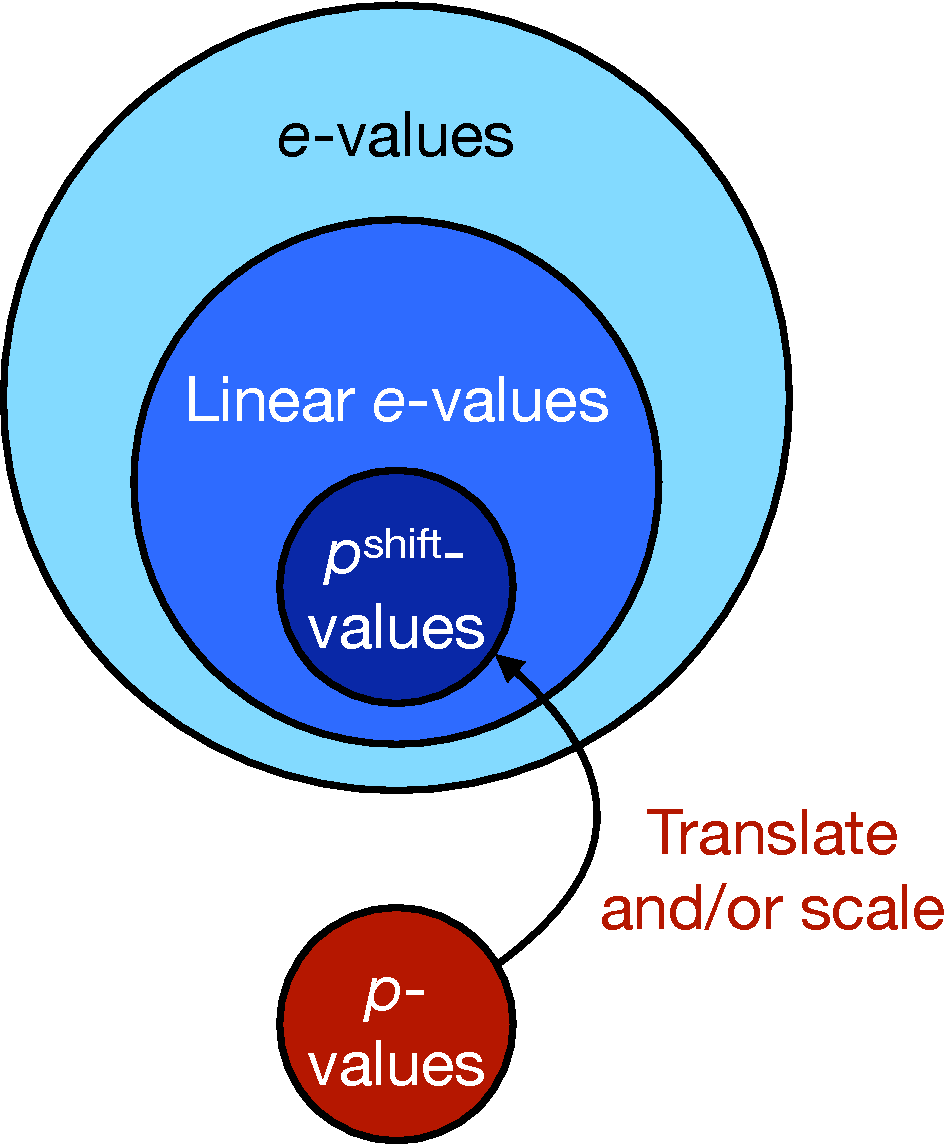
\includegraphics[width=0.4\linewidth]{test_stat_fig_crop}
	\caption{Connection between the various test statistics considered in this proposal: $p^\textrm{shift}$-values $\subset$ linear $e$-values $\subset$ $e$-values. Meanwhile, $p^\textrm{shift}$-values are scaled and/or translated $p$-values with unit expectation.}
	\label{fig:test_stats}
\end{figure}


\section*{Direction 2: A class of fast and powerful test statistics for randomization tests}
Coming soon...

\section*{Tertiary directions}
We note several possible other directions that could be of interest.
\\ \\ \noindent
1. \textbf{An analog of Selective SeqStep for $e$-values.}  Selective SeqStep is a multiple testing correction procedure for controlling FDR proposed by Barber and Candes (\cite{Barber2015}). Li and Candes recommend using Selective SeqStep instead of BH to correct $p$-values outputted by the CRT, as Selective SeqStep better handles discrete $p$-values (\cite{Li2021}). Wang and Ramdas developed an analog of BH for $e$-values; might it be possible to develop an analog of Selective SeqStep for $e$-values? Such an extension would enable users of the proposed framework to choose between different multiple testing correction procedures, which would be helpful.
\\ \\ \noindent
2. \textbf{Testing and training on the same data.} Our goal in applying the CRT is to test for conditional independence of $X$ and $Y$ given $Z$. Under what conditions can we train the regression function $\hat{E}(X|Z)$ and test the conditional independence hypothesis using the same data? Intuitively, the variance of the regression function $\hat{E}(X|Z)$ must be small. Can we derive a practical (e.g., bootstrap-based) methodology to help users determine whether or not to sample split?
\\ \\ \noindent
3. \textbf{Double robustness and double regression.} Under the right choice of the test statistic, the CRT is doubly-robust in an asymptotic (i.e., large $n$, fixed $p$) regime. Can we derive more precise, non-asymptotic or high-dimensional statements about double robustness a la double machine learning (DML; \cite{Chernozhukov2018}) or the generalized covariance measure (GCM; \cite{Shah2020})? More generally, CRT, GCM, and DML at their core are methods for causal inference based on flexible double regression. What are the connections and relative strengths and weaknesses of these approaches?
\\ \\ \noindent
4. \textbf{Theory for $p$-value vs.\
 $e$-value calibration}. It is known that exchangeability of the resampled test statistics implies implies validity of the resulting $p$-value. Can we answer the following questions? (i) Is exchangeability \textit{necessary} for the $p$-value to be valid? (ii) What are the conditions under which an $e$-value is valid? In particular, does $e$-value validity require exchangeability? Intuitively, we can construct the $e$-value in such a way that only some (rather than all) quantiles of the distribution are used. (iii) Is it possible for us to obtain a bound on the type-I error of an $e$-value a la \textcite{Berrett2020} or \textcite{Kim2021}? This statement might be in terms of expectation rather than probability.
\\ \\ \noindent
5. \textbf{The local holdout permutation test}. A simple, new conditional independence test that results from combining the holdout randomization test \parencite{Tansey2021a} with the local permutation test \parencite{Kim2021} is what I call the ``local holdout permutation test.'' The idea is as follows: (1) split the data in half, (2) train a classifier on the first half, (3) run the local permutation test on the second half, using empirical risk as the test statistic.
\\ \\ \noindent
6. \textbf{Extensions to other rank-based tests}. Can we extend the ideas here to other rank-based tests? For example, the Mann-Whitney U test, whose test statistics basically is a sum of ranks?

 % \textbf{NOTE}: I (Tim) know that Nav and Gene already are working on the double robustness problem. I do not want to duplicate effort!

\printbibliography
\begin{appendices}
\subsection*{Proposition 2 proof}
Define the set $C(r,B)$ by
$$C(r,B) := \left\{ (k_1, \dots, k_B) \in \{0, \dots, r\}^B : \sum_{i=1}^B k_i = r \right\},$$ i.e., $C(r,B)$ is the set of length-$B$ tuples of integers from $0$ to $r$ such that the elements of the tuple sum to $r$. Next, let the function $\tau: C(r,B) \to \{ 1, \dots, B \}$ be defined by
$$ \tau(k_1, \dots, k_B) = \min\left\{ i \in \{ 1, \dots, B \} : k_i \geq 1 \right\},$$
i.e., $\tau(k_1, \dots, k_B)$ is the position of the minimal nonzero element of a $(k_1, \dots, k_B)$. Finally, let $\tau^{-1}$ be the pre-image of of $\tau$. It is easy to see that, for $i \in \{0, \dots, B\}$,
$$\tau^{-1}(i) = \{ (0, \dots, 0, k_i, k_{i+1}, \dots, k_B) \in C(r,B) : k_i \geq 1 \}.$$ In other words, $\tau^{-1}(i)$ is the set of tuples whose first nonzero entry is the $i$th entry. 

Before proceeding, we establish an important property of the $I_i$s. If at least one of the $k_i$s is nonzero, we have that
\begin{equation}\label{pf_res}
 \prod_{i=1}^B I^{k_i}_i = I_{\tau(k_1, \dots, k_B)}.
 \end{equation}
This equality holds for the following reason. Assume without loss of generality that there are $N \in \{1, \dots, B\}$ nonzero $k_i$s. Let $\sigma: \{1, \dots, N\} \to \{1, \dots, B\}$ give the position of the $i$th nonzero $k_i$ (so that $\sigma(1)$ is the position of the first nonzero $k_i$, $\sigma(2)$ is the position of the second, etc.). We can write
\begin{equation}\label{pf_1}
\prod_{i=1}^B I_i^{k_i} = \prod_{i=1}^N I_{\sigma(i)}^{k_{\sigma(i)}},
\end{equation} 
i.e., we can remove all $I_i$s that are raised to the power of zero. Because the $I_i$s are Bernoulli random variables, we have that $I_{\sigma(i)}^{ k_{\sigma(i)}} = I_{\sigma(i)}$. Next, recall that $I_\sigma(i) = \mathbb{I}\left( T^* \leq T_{\sigma(i)} \right)$, where $T_{\sigma(1)} < T_{\sigma(2)} < \dots < T_{\sigma(n)}.$ If $T^* \leq T_{\sigma(i)}$, then by transitivity, $T^* \leq T_{\sigma(2)} < \dots < T_{\sigma(n)}$, implying $I_{\sigma(i)} = 1$ for all $i \in \{1, \dots, N\}.$ Therefore, $I_{\sigma(1)} = 1 = I_{\sigma(1)} \dots I_{\sigma(n)}.$ On the other hand, if $T^* > T_{\sigma(i)}$ then $T_{\sigma(1)} = 0,$ implying $I_{\sigma(1)} = 0 = I_{\sigma(1)} \dots I_{\sigma(n)}$. Combining these cases, we conclude that $I_{\sigma(1)} = I_{\sigma(1)} \dots I_{\sigma(B)}$. Equation \ref{pf_1} therefore reduces to
\begin{equation}\label{pf_2}
\prod_{i=1}^N I_{\sigma(i)}^{k_{\sigma(i)}} = I_{\sigma(1)}.
\end{equation}
 Finally, because $\sigma(1)$ is the position of the first nonzero $k_i$, we have that $\sigma(1) = \tau(k_1, \dots, k_B).$ Combining this fact with (\ref{pf_1}) and (\ref{pf_2}) yields the conclusion (\ref{pf_res}).

Having established this lemma, we can evaluate the $r$th power of the sum of the $I_i$s. The multinomial theorem states that
\begin{multline}\label{pf_3}
\left( \sum_{i=1}^B I_i \right)^r = \sum_{(k_1, \dots, k_B):k_1 + \dots + k_B = r} \binom{ r }{k_1, k_2, \dots, k_B} \prod_{i=1}^B I^{k_i}_i \\ = \sum_{(k_1, \dots, k_B):k_1 + \dots + k_B = r} \binom{r}{k_1, k_2, \dots, k_B} I_{\tau(k_1, \dots, k_B)},
\end{multline}
where the second equality follows from (\ref{pf_res}). The final term in (\ref{pf_3}) is simply a linear combination of the $I_i$s. We therefore can factor out the terms in the sum corresponding to $I_i$ for each $i$, yielding
\begin{multline}\label{pf_4}
\sum_{(k_1, \dots, k_B):k_1 + \dots + k_B = r} \binom{r}{k_1, k_2, \dots, k_B} I_{\tau(k_1, \dots, k_B)} = \sum_{i=1}^B \sum_{(k_1, \dots, k_B) \in \tau^{-1}(i)} \binom{r}{k_1, k_2,\dots, k_B} I_i \\ = \sum_{i=1}^B I_i \sum_{ (k_1, \dots, k_B) \in \tau^{-1}(i)} \binom{r}{k_1, k_2,\dots, k_B}.
\end{multline}
We evaluate the inner sum (\ref{pf_4}), which is the coefficient corresponding to $I_i$ in the linear combination. We have that
\begin{multline}\label{pf_5}
 \sum_{ (k_1, \dots, k_B) \in \tau^{-1}(i)} \binom{r}{k_1, k_2,\dots, k_B} =  \sum_{( 0, \dots, 0, k_i, \dots, k_B): k_i \geq 1, k_i + \dots + k_B = r} \binom{r}{k_1, k_2, \dots, k_B} \\ = \sum_{(k_1, \dots, k_{B - i + 1}) : k_1 \geq 1, k_1 + \dots + k_{B - i + 1} = r} \binom{r}{k_1, k_2, \dots, k_{B - i + 1} } = \sum_{j=1}^r \sum_{l_1 + \dots + l_{B - i} = r - j} \binom{r}{ j, l_1, \dots, l_{B-i}} \\ = \sum_{j=1}^r \sum_{ l_1 + \dots + l_{B-i} = r-j } \frac{ r! }{ j! l_1! \dots l_{B-i}!} = \sum_{j=1}^r \sum_{l_1 + \dots + l_{B-i} = r-j} \frac{r(r-1)\dots(r-j+1)(r-j)!}{ j! l_1! \dots l_{B-i}!}  \\ = \sum_{j=1}^r \sum_{l_1 + \dots + l_{B-i} = r - j} \frac{r!}{(r-j)!j!} \binom{r-j}{l_1, \dots, l_{B-i}} = \sum_{j=1}^r \frac{r!}{(r-j)!j!} \sum_{l_1, \dots, l_{B-i}} \binom{r-j}{l_1, \dots, l_{B-i}} \\ = \sum_{j=1}^r \binom{r}{j} (B-i)^{r-j}  = \sum_{j=1}^r \binom{r}{j} (B-i)^{r-j} 1^j = \sum_{j=0}^r \binom{r}{j} (B-i)^{r-j}1^j  - 1(B-i)^r \\ = (B - i + 1)^r - (B-i)^r.
\end{multline}
Combining (\ref{pf_3}), (\ref{pf_4}), and (\ref{pf_5}), we conclude that
$$ \left( \sum_{i=1}^B I_i \right)^r = \sum_{i=1}^B \left[ (B - i + 1)^r - (B - i)^r \right] I_i.$$
Next, setting $p_B = \frac{1}{B} \sum_{i=1}^B I_i$, we obtain
$$p^r_B = \left( \frac{1}{B}\sum_{i=1}^B I_i \right)^r = \sum_{i=1}^B \left[ (1 - i/B + 1/B)^r - (1 - i/B)^r \right] I_i = \sum_{i=1}^B M(B,r,i) I_i.$$ We next consider the $r$th degree polynomial of $p^r_B$. First, for $j \in \N$, and $x_0 \in \R$, we have that
\begin{multline*}
\left(p_B - x_0 \right)^j = \sum_{k=0}^j \binom{j}{k} p_B^k x_0^{j-k}(-1)^{j-k} = x^j_0(-1)^j + \sum_{k=1}^j \binom{j}{k}p_B^k x_0^{j - k}(-1)^{j-k} \\ = x^j_0(-1)^j + \sum_{k=1}^j \binom{j}{k} \left[\sum_{i=1}^B M(B,k,i) I_i \right] x^{j-k}_0(-1)^{j-k} \\ = x^j_0(-1)^j + \sum_{i=1}^B  \left[ \sum_{k=1}^j x_0^{j-k} \binom{j}{k} (-1)^{j-k} M(B,k,i) \right] I_i.
\end{multline*}
Finally, let $c_0, c_1, \dots, c_r \in \R$ be polynomial coefficients. We have that
\begin{multline*}
\sum_{j=0}^r c_j \left(p_B - x_0 \right)^j  = c_0 + \sum_{j=1}^r c_j (p_B - x_0)^j \\ = c_0 + \sum_{j=1}^r c_j \left[x_0^j(-1)^j + \sum_{i=1}^B \left[\sum_{k=1}^j x_0^{j-k} \binom{j}{k}(-1)^{j-k} M(B,k,i) \right] I_i \right] \\ = \sum_{j=0}^r c_j x_0^j(-1)^j + \sum_{i=1}^B \left[\sum_{j=1}^r \sum_{k=1}^j c_j x_0^{j-k} \binom{j}{k} (-1)^{j-k} M(B,k,i) \right] I_i,
\end{multline*}
completing the proof.

\section{Beginning theory on calibration}

Let $W_1, \dots, W_n$ be exchangeable. For $t \in \R$, we have that
$$ \P( \textrm{rank}(W_n) \leq t) = \frac{\lfloor t \rfloor}{n}.$$ Define $P_n := \textrm{rank}(W_n)/n.$ Then
$$ \P( P_n \leq \alpha) = \P( \textrm{rank}(W_n)/n \leq \alpha) = \P( \textrm{rank}(W_n) \leq n\alpha ) = \frac{ \lfloor n \alpha \rfloor }{ n } \leq \frac{n\alpha}{n} = \alpha.$$ Therefore, $P_n$ is a valid $p$-value. Moreover, $P_n$ converges in distribution to $U[0,1]$, i.e.,
$$ \lim_{n \to \infty} \P(P_n \leq \alpha) = \alpha.$$ By way of proof, let $\ep > 0$ be given. Let $N = 1/\ep$, and let $n > N$ for $n \in \N$. Then
$$
\left| \alpha - \frac{ \lfloor n \alpha \rfloor }{ n } \right| = \left| \frac{n\alpha}{n} - \frac{ \lfloor n \alpha \rfloor }{ n } \right| \leq 1/n \textrm{ (because $x - \lfloor x \rfloor \leq 1$ )} < \ep.
$$
Conversely, let $(W_1, \dots, W_n)$ be a sequence of random variables. Define $P_n := \textrm{rank}(W_n)/n$, as before. Assume that
$$ \lim_{n \to \infty} \P\left( P_n \leq \alpha \right) = \lim_{n\to\infty}\P(\textrm{rank}(W_n)/n \leq \alpha) = \alpha.$$ We want to show that $(W_1, \dots, W_n)$ are exchangeable.


\end{appendices}
\end{document}
